% ===========================================================================
%  E-Trike SYS ESP32-S3: Controls & 12 V Relay Wiring Reference Sheet
%  Professional Engineering Reference | Clean Single-Page Layout
%  Compile: pdflatex -interaction=nonstopmode sys-controls-wiring.tex
% ===========================================================================
\documentclass[10pt,a4paper]{article}

\usepackage[utf8]{inputenc}
\usepackage[T1]{fontenc}
\usepackage{lmodern}
\usepackage[margin=8.5mm,footskip=0mm]{geometry}
\usepackage{booktabs}
\usepackage{array}
\usepackage{tabularx}
\usepackage{xcolor}
\usepackage{colortbl}
\usepackage{tikz}
\usetikzlibrary{shapes,arrows.meta,positioning,calc}
\usepackage[most]{tcolorbox}
\usepackage{hyperref}

\pagestyle{empty}

% ── Color Palette ──────────────────────────────────────────────────────────
\definecolor{brandNavy}{HTML}{0F172A}
\definecolor{brandBlue}{HTML}{1D4ED8}
\definecolor{cardBg}{HTML}{F8FAFC}
\definecolor{cardBorder}{HTML}{CBD5E1}
\definecolor{accentRed}{HTML}{DC2626}
\definecolor{accentGreen}{HTML}{16A34A}
\definecolor{accentAmber}{HTML}{D97706}
\definecolor{tableStripe}{HTML}{F1F5F9}

\hypersetup{
  colorlinks=true,
  linkcolor=brandBlue,
  urlcolor=brandBlue,
  pdftitle={SYS ESP32-S3 Controls and Relay Wiring Reference},
  pdfauthor={E-Trike Safety Systems},
}

% ── Custom Card Styles ─────────────────────────────────────────────────────
\tcbset{
  basecard/.style={
    enhanced,
    colback=cardBg,
    colframe=cardBorder,
    boxrule=0.7pt,
    arc=3pt,
    left=6pt, right=6pt, top=5pt, bottom=5pt,
    fonttitle=\bfseries\small\color{white},
    coltitle=white,
    attach boxed title to top left={yshift*=-\tcboxedtitleheight/2, xshift=8pt},
    boxed title style={
      colback=brandNavy,
      colframe=brandNavy,
      arc=2pt,
      boxrule=0pt,
      top=2pt, bottom=2pt, left=6pt, right=6pt
    }
  }
}

\begin{document}

% ── Header Banner ──────────────────────────────────────────────────────────
\begin{tcolorbox}[
  enhanced,
  colback=brandNavy,
  colframe=brandNavy,
  arc=3pt,
  boxrule=0pt,
  left=8pt, right=8pt, top=4pt, bottom=4pt
]
\begin{tabularx}{\textwidth}{@{}X r@{}}
  {\bfseries\color{white}\fontsize{11.5}{13}\selectfont E-TRIKE: SYS ESP32-S3 CONTROLS \& 12\,V RELAY WIRING} & \textbf{\small\color{cardBorder} REV 0.8.0-ALPHA} \\
  {\footnotesize\color{cardBorder} Master Safety Authority $\cdot$ Pilot Controls $\cdot$ Body Relay Drivers} & {\footnotesize\color{cardBorder} Active-GND Inputs $\cdot$ 3.3\,V Internal Pull-Ups} \\
\end{tabularx}
\end{tcolorbox}

\vspace{-4pt}

% ── Invariant Alert Bar ────────────────────────────────────────────────────
\begin{tcolorbox}[
  enhanced,
  colback=accentRed!7!white,
  colframe=accentRed!80!black,
  boxrule=0.8pt,
  arc=2pt,
  left=6pt, right=6pt, top=3pt, bottom=3pt
]
\footnotesize
\textbf{\color{accentRed}CRITICAL ELECTRICAL RULES:}
\textbf{1.} All pilot switches \& buttons switch directly to \textbf{GND (0\,V)} using MCU internal pull-ups.
\textbf{2.} \textbf{NEVER connect +12\,V or external 3.3\,V to any ESP32 GPIO.}
\textbf{3.} ESTOP loop is \textbf{Normally Closed (NC) to GND}; open/broken wire = immediate fail-safe ESTOP.
\end{tcolorbox}

\vspace{-3pt}

% ── Section 1: Switches & Digital Inputs ────────────────────────────────────
\begin{tcolorbox}[basecard, title={1. Pilot Switches \& Digital Inputs (Dry Contact to GND)}]
\vspace{1pt}
\footnotesize
All digital inputs utilize ESP32-S3 \textbf{internal pull-ups (to 3.3\,V)}. Wire dry contacts between GPIO and common \textbf{GND}. No external resistors required.

\vspace{2pt}
\begin{tabularx}{\textwidth}{@{} l c l l X @{}}
\toprule
\textbf{Function} & \textbf{GPIO} & \textbf{Contact Type} & \textbf{Electrical State} & \textbf{Firmware / Safety Action} \\
\midrule
\rowcolor{tableStripe}
\textbf{ESTOP Button} & \textbf{GPIO 1} & \textbf{NC Red Mushroom} & Closed = 0\,V (Healthy) & Open / Cut = 3.3\,V $\rightarrow$ Immediate Latched ESTOP \\
\textbf{Brake Lever} & \textbf{GPIO 2} & NO Limit Microswitch & Closed = 0\,V (Active) & Overrides throttle $\rightarrow$ Demands SEB brake (0x7B9) \\
\rowcolor{tableStripe}
\textbf{START Button} & \textbf{GPIO 41} & Momentary NO Push Button & Pressed = 0\,V & Exits ESTOP $\rightarrow$ MANUAL mode (500\,ms debounce) \\
\textbf{MODE Button} & \textbf{GPIO 11} & Momentary NO Push Button & Pressed = 0\,V & Short: MANUAL $\leftrightarrow$ AUTO; Hold 3s: Exits ESTOP \\
\rowcolor{tableStripe}
\textbf{Bypass Mode} & \textbf{GPIO 42} & Latching Switch / Jumper & Closed to GND = ON & Enables developer bench solo bypass mode at boot \\
\textbf{Left Turn Sw} & \textbf{GPIO 9} & Handlebar Push / Toggle & Pressed = 0\,V & Toggles left turn signal flasher in MANUAL mode \\
\rowcolor{tableStripe}
\textbf{Right Turn Sw} & \textbf{GPIO 6} & Handlebar Push / Toggle & Pressed = 0\,V & Toggles right turn signal flasher in MANUAL mode \\
\textbf{Headlight Sw} & \textbf{GPIO 7} & Handlebar Toggle Switch & Closed = 0\,V & Toggles headlight output in MANUAL mode \\
\bottomrule
\end{tabularx}
\end{tcolorbox}

\vspace{-3pt}

% ── Section 2: 12V Relay Module & Indicators ─────────────────────────────────
\begin{tcolorbox}[basecard, title={2. 12\,V Relay Outputs \& Dashboard Lamps}]
\vspace{1pt}
\footnotesize
Drives an 8-channel \textbf{Active-LOW} 12\,V relay board via a \textbf{ULN2803A Darlington sink array} (ESP32 $\rightarrow$ ULN $\rightarrow$ Relay INx).

\vspace{2pt}
\begin{tabularx}{\textwidth}{@{} l c l l X @{}}
\toprule
\textbf{Indicator / Load} & \textbf{ESP32} & \textbf{ULN2803A} & \textbf{Relay Channel} & \textbf{Indication \& Logic} \\
\midrule
\rowcolor{tableStripe}
\textbf{Bulb AUTO} & GPIO 48 & IN1 $\rightarrow$ OUT1 & Relay 1 (K1) & High (ON) when vehicle is in \textbf{AUTO} mode \\
\textbf{Bulb MANUAL} & GPIO 39 & IN2 $\rightarrow$ OUT2 & Relay 2 (K2) & High (ON) when vehicle is in \textbf{MANUAL} mode \\
\rowcolor{tableStripe}
\textbf{Bulb READY} & GPIO 17 & IN3 $\rightarrow$ OUT3 & Relay 3 (K3) & Green lamp: RT alive, heartbeat healthy, no faults \\
\textbf{USB Data+} & GPIO 20 & IN4 $\rightarrow$ OUT4 & Relay 4 (K4) & \textit{\color{accentRed}DO NOT USE / LEAVE UNCONNECTED (ESP32 USB D+)} \\
\rowcolor{tableStripe}
\textbf{Bulb BYPASS} & GPIO 14 & IN5 $\rightarrow$ OUT5 & Relay 5 (K5) & Amber lamp: Developer bench bypass active \\
\textbf{Bulb ESTOP} & GPIO 18 & IN6 $\rightarrow$ OUT6 & Relay 6 (K6) & \textbf{Red lamp:} Hard or soft ESTOP latched \\
\rowcolor{tableStripe}
\textbf{USB Data$-$} & GPIO 19 & IN7 $\rightarrow$ OUT7 & Relay 7 (K7) & \textit{\color{accentRed}DO NOT USE / LEAVE UNCONNECTED (ESP32 USB D-)} \\
\textbf{Brake Lamp} & GPIO 21 & IN8 $\rightarrow$ OUT8 & Relay 8 (K8) & 12\,V Rear Brake Light (Lever $\lor$ ESTOP $\lor$ SEB active) \\
\bottomrule
\end{tabularx}
\end{tcolorbox}

\vspace{-3pt}

% ── Section 3: Visual Topologies ──────────────────────────────────────────
\begin{tcolorbox}[basecard, title={3. Circuit Topologies \& Power Distribution}]
\vspace{1pt}
\begin{tabularx}{\textwidth}{@{} X X @{}}
  \textbf{(A) Switch Input Circuit (to GND):} & \textbf{(B) 12\,V Relay Driver Chain:} \\
  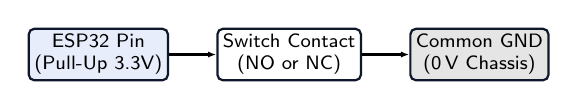
\begin{tikzpicture}[
    node distance=0.8cm and 0.9cm,
    font=\scriptsize\sffamily,
    box/.style={draw=brandNavy, fill=white, rounded corners=2pt, minimum height=16pt, align=center, inner sep=2pt, thick},
    wire/.style={thick, -{Latex[length=3pt]}}
  ]
    \node[box, fill=brandBlue!10] (esp) {ESP32 Pin\\(Pull-Up 3.3V)};
    \node[box, right=0.6cm of esp] (sw) {Switch Contact\\(NO or NC)};
    \node[box, fill=black!10, right=0.6cm of sw] (gnd) {Common GND\\(0\,V Chassis)};
    \draw[wire] (esp) -- (sw);
    \draw[wire] (sw) -- (gnd);
  \end{tikzpicture}
  &
  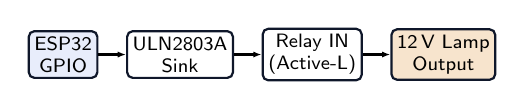
\begin{tikzpicture}[
    node distance=0.5cm,
    font=\scriptsize\sffamily,
    box/.style={draw=brandNavy, fill=white, rounded corners=2pt, minimum height=16pt, align=center, inner sep=2pt, thick},
    wire/.style={thick, -{Latex[length=3pt]}}
  ]
    \node[box, fill=brandBlue!10] (gpio) {ESP32\\GPIO};
    \node[box, right=0.35cm of gpio] (uln) {ULN2803A\\Sink};
    \node[box, right=0.35cm of uln] (ry) {Relay IN\\(Active-L)};
    \node[box, fill=accentAmber!20, right=0.35cm of ry] (lp) {12\,V Lamp\\Output};
    \draw[wire] (gpio) -- (uln);
    \draw[wire] (uln) -- (ry);
    \draw[wire] (ry) -- (lp);
  \end{tikzpicture}
  \\
  \midrule
  \textbf{Relay Contact Wiring:} & \textbf{Common Grounds:} \\
  $\bullet$ +12\,V Fused $\rightarrow$ Relay COM terminal & $\bullet$ ESP32 GND = ULN GND = Relay GND \\
  $\bullet$ Relay NO $\rightarrow$ Lamp (+) $\quad\vert\quad$ Lamp ($-$) $\rightarrow$ GND & $\bullet$ Common vehicle chassis ground (0\,V) \\
\end{tabularx}
\end{tcolorbox}

\end{document}
